\documentclass{bio}
%\documentclass[oupdraft]{bio}
\usepackage[colorlinks=true, urlcolor=citecolor, linkcolor=citecolor, citecolor=citecolor]{hyperref}
\usepackage[utf8]{inputenc}
\usepackage[english]{babel}

% Add history information for the article if required
%\history{}


%% NOTES TO SELF:
% Cite using:
%    \citet{...}  in text
%    \citealp{...}   within parantheses
%
% Temporary notifications and reminders:
\newcommand\NB[1]{{\color{red}#1}}
\newcommand\NOTE[1]{{\color{red}[#1]}}
\newcommand\CITE[1]{{\color{magenta}[#1]}}


\begin{document}

% Title of paper
\title{Methods that remove batch effects while retaining group differences may lead
to exaggerated confidence in downstream analyses
}

% List of authors, with corresponding author marked by asterisk
\author{VEGARD NYGAARD, EINAR ANDREAS RØDLAND, EIVIND HOVIG$^\ast$\\[4pt]
% Author addresses
\textit{Department of Tumor Biology,
Institute for Cancer Research,
Oslo University Hospital HF - Radiumhospitalet,
Montebello,
0310 Oslo,
Norway}
\\[2pt]
% E-mail address for correspondence
{ehovig@ifi.uio.no}}


% Running headers of paper:
\markboth%
% First field is the short list of authors
{V. Nygaard, E. A. Rødland, E. Hovig}
% Second field is the short title of the paper
{Exaggerated effects after batch correction}


\maketitle


% Add a footnote for the corresponding author if one has been
% identified in the author list
\footnotetext{To whom correspondence should be addressed.}

\begin{abstract}
{Removal of, or adjustment for, batch effects or centre differences is generally required when such effects are present in data. In particular, when preparing microarray gene expression data from multiple cohorts, array platforms, or batches for later analyses, batch effects can have confounding effects. Many methods and tools exist for this purpose. One method, ComBat which is part of the R package sva, is particularly popular due to its ability to remove batch differences even when batches are small and heterogeneous. It also has the option of preserving the difference between study groups, estimated from a two-way ANOVA model, to avoid conflating batch effects and group differences during batch adjustments. Unfortunately, this frequently used and recommended approach may systematically induce incorrect group differences in downstream analyses when groups are distributed between the batches in an unbalanced manner. The scientific community seems to be largely unaware of this problem, which most likely has contributed to false discoveries being presented in the published literature.
}
\end{abstract}


\section{Introduction}\label{intro}

Extraneous variables, if left unaccounted for, have the potential to lead an investigator into drawing wrong conclusions. In molecular biology, extraneous variables are often called "batch effects", probably due to the fact that reagents and other equipment, for instance microarray chips, are made in batches, and this is frequently observed as an effect in the measurements. See \citet{Luo2010} for more examples. 

For a typical experiment comparing group differences, the presence of batch effects will decrease the statistical power since it adds variation to the data. If the batch--group design is unbalanced, i.e if the study groups are not equally represented in all batches, batch effects may act as a confounder and induce false differences between groups (\citealp{Leek2010}).

The standard way to handle an extraneous variable is to include it in the statistical model employed in the inquiry. However, many analysis tools for high throughput data do not cater for this option, and when available it could still be outside the competence of the investigator. Therefore, an alternative two step procedure has emerged. First the batch effects are estimated and removed, creating a ``batch effect free'' data set. In the next step, the statistical analyses are performed on the adjusted data without further consideration of batch effects. This appealing compartmentalization is also convenient for practical purposes, for example when data-processing and statistical analyses are performed by different personnel.

The first step can be achieved by subtracting the mean of the measurements in one batch from all measurements in that batch, i.e mean adjustment or one-way ANOVA adjustment as implemented in the method \texttt{pamr.batchadjust} from the \texttt{pamr} package in R. When the batch--group design is balanced, mean-adjustment will remove most, but not necessarily all, variance attributed to batch and leave the between group variance, thus increasing the statistical power. However, when the batch--group design is unbalanced, batch differences will in part be influences by group differences, and thus batch correction will reduce group differences and thereby reduce the statistical power. In very uneven group--batch designs with multiple groups, spurious group differences may even be induced in this way. Figure~\ref{fig:boxplots} illustrates both these effects.

To mitigate the above problems, one may simultaneously estimate batch effects and group differences, e.g. using a two-way ANOVA, and only remove the batch differences from the data. Effectively, this means group differences are estimated based on within batch comparison, and applied to the batch adjusted data. In a balanced group--batch design, group differences and batch effects are independent, and this approach becomes identical to the above described zero-centering per batch. If the group--batch design is heavily unbalanced, estimation of group differences and batch effects are interdependent. Unfortunately, when group differences estimated from an unbalanced group--batch design are applied to the entire data set, if this batch adjusted data set is later analysed for group differences, the confidence will be exaggerated as the estimation of the group differences in the unbalanced design is less accurate than in the corresponding balanced design. Figure~\ref{fig:boxplots} illustrates how statistical uncertainties are deflated by this batch adjustment method by comparing them to the uncertainties from the original ANOVA.

The ComBat method described in \citet{Johnson2007}, and included in the sva package (\citealp{Leek2012}), can use either of the two above described approaches to estimate batch differences, but uses an empirical Bayes approach to avoid over-correction for batch effects for small batches. It has popularised the two-way ANOVA procedure for retaining group differences when adjusting for batch effects, and the inclusion of group difference as a covariate when removing batch effects has been recommended in the sva tutorial and user fora. Based on actual use of ComBat by the authors and others, ourselves included, we suspect thus adjusted data are commonly treated as "batch effect free" in subsequent analyses. And as a consequence, confidence in group effects has been overestimated and false results reported.

\section{Methods for batch effect correction}

\subsection{Model for data with batch effects}

We will base our discussion of data with batch effects on a simple model:
\begin{equation}
Y_{ijr}=\alpha+\beta_j+\gamma_i+\epsilon_{ijr}
\end{equation}
where $i=1,\ldots,m$ are the different batches, $j=1,\ldots,M$ are different study groups that we wish to compare, and $r=1,\ldots,n_{ij}$ are the different samples within batch $i$ and group $j$.

When combining data from more diverse data sources, e.g. microarray data from different platforms, a more general model is required. One such model, used by \citet{Johnson2007}, is
\begin{equation}
Y_{ijgr}=\alpha_g+X_r\beta_{g}+\gamma_{ig}+\delta_{ig}\epsilon_{ijgr}
\end{equation}
where $g=1,\ldots,G$ are different measurements, e.g. genes, performed for each sample, and $X$ is the design matrix which in our case will indicate the study group. This permits independent rescaling of data from different batches. In addition, \citet{Johnson2007} uses an empirical Bayes approach to estimate $\gamma_{ig}$ and $\delta_{ig}$ to stabilise estimates, which is critical for use with small batches.

For simplicity, we consider the case with a single gene and constant scale, i.e. $\delta_{ig}=1$. We will discuss the effect of empirical Bayes estimation of $\gamma_{ig}$ later, but out main argument is more easily made in the simpler context.

\subsection{Standard batch correction methods}

The main ambition of batch effect adjustments is to be able to remove batch differences in such a way that downstream analyses of the adjusted data may be done without further batch adjustments.

The most common method for removing batch effects is to zero-centre each batch:
\begin{equation}
\Delta\widetilde Y_{ijr}=Y_{ijr}-\bar{Y}_{i}
\quad\text{where}\quad
\bar{Y}_i=\frac{\sum_{j=1}^M\sum_{r=1}^{n_{ij}} Y_{ijr}}{\sum_{j=1}^M n_{ij}}.
\end{equation}
An alternative is to centre each batch to the common average by adding the average value $\bar{Y}$ across the entire data set: i.e. $\widetilde Y_{ijr}=\Delta\widetilde Y_{ijr}+\bar{Y}$. When comparing groups, the common value $\bar{Y}$ has no effect, and so this is equilvalent to zero-centring each batch. However, if the different groups are unevenly represented in the different batches, the batch average $\bar{Y}_i$ will tend to capture group differences as well as batch effects. Thus, batch centering may reduce group differences, and thus reduce the power of downstream analyses.

Removing batch effects while retaining group differences can be done through an ANOVA analysis in which the group effects, $\beta_j$, and the batch effects, $\gamma_i$, are estimated simultaneously. Batch adjusted values may then be obtained by subtracting the estimated batch effects, $\hat\beta_j$:
\begin{equation}
\widetilde Y_{ijr}=Y_{ijr}-\hat\beta_j=\alpha+(\beta_j-\hat\beta_j)+\gamma_i+\epsilon_{ijr}.
\end{equation}
This will yield batch adjusted values where any systematic bias induced by the batch differences has been removed, while the group differences are retained.

Unfortunately, the estimation error $\hat\beta_j-\beta_j$ affects all values within the same batch in the same manner, inducing a dependency between the values. If the study groups are evenly represented in all batches, this will not influence estimated group differences as all groups are equally affected. However, if groups are unevenly represented, this induced dependency can have severe impact on downstream analyses.


\section{Results}

\subsection{A simple sanity check}

The undesired consequences of preserving group effects when correcting for batch effect is readily illustrated with a sanity check using random numbers . The documentation accompanying the sva library has a runnable example demonstrating how to adjust a data set with ComBat followed by a F-test. Swapping the real data with random numbers from a normal distribution (mean=0, sd=1), but otherwise following the instructions, will generate the p-value distribution shown in Figure 1. The skewed distribution is a indication that this approach may have a unintentional adverse effect. 

%% FIGURE 1: Original position

\subsection{Explanation for the simple two-group comparison}

To explain more clearly what is happening, and quantify the size of the problem, we may consider the simple case of estimating the difference $\Delta\beta=\beta_A-\beta_B$ between two groups, $A$ and $B$, when there are $m$ batches with batch $i$ containing $n_{iA}$ and $n_{iB}$ samples from each of the two groups for $i=1,\ldots,m$.

If we estimate the group difference within batch $i$, we get
\begin{equation}
\widehat{\Delta\beta}_i=\bar{Y}_{iA}-\bar{Y}_{iB}\sim\text{N}\left(\Delta\beta,\frac{\sigma^2}{\nu_i}\right)
\quad\text{where}\quad
\bar{Y}_{ij}=\frac{\sum_{r=1}^{n_{ij}}Y_{ijr}}{n_{ij}},\,
\nu_i=\frac{1}{\frac{1}{n_{iA}}+\frac{1}{n_{iB}}},
\end{equation}
from which we may express the overall estimate of $\Delta\beta$
\begin{equation}
\widehat{\Delta\beta}=\frac{\sum_{i=1}^m \nu_i\,\widehat{\Delta\beta}_i}{\nu}
\sim\text{N}\left(\Delta\beta,\frac{\sigma^2}{\nu}\right)
\quad\text{where}\quad
\nu=\sum_{i=1}^m\nu_i.
\end{equation}

If batch and group effects are estimated using a two-way ANOVA, the estimate $\widehat{\Delta\beta}$ will be as stated above, and so the estimated group difference is unaffected. The batch effects are then removed, and the estimated group differences retained, leaving the estimated $\widehat{\Delta\beta}$ unchanged by the batch adjustment. However, if this batch adjusted data set is analysed without considering batch effects, the variance of $\widehat{\Delta\beta}$ will be computed under the assumption that it is derived from a comparison of $n_A=\sum_{i=1}^m n_{iA}$ versus $n_B=\sum_{i=1}^m n_{iB}$ samples, and thus satisfy
\begin{equation}
\widehat{\Delta\beta}
\sim\text{N}\left(\Delta\beta,\sigma^2\cdot\left(\frac{1}{n_A}+\frac{1}{n_B}\right)\right).
\end{equation}
Using Jensen's inequality, we may then derive
\begin{equation}
\frac{1}{\frac{1}{n_A}+\frac{1}{n_B}}=n\cdot\frac{n_A}{n}\cdot\frac{n_B}{n}
\le
\nu
=\sum_{i=1}^m \frac{1}{\frac{1}{n_{iA}}+\frac{1}{n_{iB}}}
=\sum_{i=1}^m n_i\cdot\frac{n_{iA}}{n_i}\cdot\frac{n_{iB}}{n_i}
\end{equation}
with equality if and only if the ratios $n_{iA}:n_{iB}=n_A:n_B$ for all batches $i=1,\ldots,m$.



\subsection{Examples of undesired consequences}

As the amount of false positive results when trying to retain group differences depends on the batch-group balance, we will show two examples with varying degree of unbalancedness. 

1) In the first experiment(\citealp{Towfic2014}), cells were treated with glatiramer acetate (a medicine for multiple sclerosis) or a generic and mRNA was measured using microarrays alongside control samples. A batch effect correlating to the chip (Illumina WG-6\_V2, six samples per chip) was observed and adjusted for with ComBat, whereafter the data was tested for differentially expressed genes, yielding a list of 1000 genes (Table S5, \citealp{Towfic2014}). Unfortunately the batch-treatment design was unbalanced with several batches having only one of the main treatments of interest. When we re-analyzed their data without using ComBat, but instead blocked for batch effect in limma, only 9 genes were found ($\text{FDR}<0.05$). The above outlined sanity check with random numbers were also performed. The distributions of p-values for different settings are shown in Fig. 3a.  Our conclusion is that most of the genes reported as differentially expressed in (\citealp{Towfic2014}) are false positives. This example is a sort of "worst case" scenario for applying ComBat, since it both has a very unbalanced batch-group design and a a priori assumption of no difference. The R-code for our analysis can be downloaded from Github (\href{https://github.com/ous-uio-bioinfo-core/batch-adjust-warning-figures.git}).

%% FIGURE 2: Original position

2) The second example is taken from the supporting information for the original ComBat article (\citealp{Johnson2007}) where it is denoted "Data Set 2". Cells inhibited for the expression of the TAL1 gene were compared to controls on a microarray platform. The experiment was conducted on three different time points (used as batches) with a total of 30 samples and a fairly balanced batch-treatment set up (6-2, 3-4 and 9-6). ComBat was applied followed by a t-test in order to identify differentially expressed genes. First, we reproduced their analysis including the adjustment by ComBat, but using limma instead of the t-test, resulting in 1003 probes ($q<0.05$).  Then, we analysed their data without batch adjustment in ComBat, but blocking for batch in limma, resulting in 377 probes ($q<0.05$). In addition, the sanity check outlined above were performed. The distributions of p-values for different settings are shown in Fig. 3b. In contrast to the results obtained for \citealp{Towfic2014} (Fig.3b) , the P-value distributions for the alternative analyses  does not indicate a huge difference. Nevertheless, we belive that  P-values are deflated for the ComBat adjusted analysis. The R-code for our analysis can be downloaded from Github (\href{https://github.com/ous-uio-bioinfo-core/batch-adjust-warning-figures.git}).

%% FIGURE 3: Original position

%% FIGURE 4: Original position

\section{Discussion}

\subsection{Increased emphasis on preserving group difference}

In the original ComBat article (\citealp{Johnson2007}) it is clear that the primary motivation behind ComBat was to employ an Emprical Bayes method for batch-effect removal. The feature of retaining group differences for unbalanced designs is optional and seems to be subordinate, only exemplified in the supplementary information. However, over the years this feature became more important judging from advice given on user fora. And when ComBat was incorporated in the sva package (\citealp{Leek2012}), inclusion of group labels was made almost mandatory (an undocumented option of passing a NULL value exists). Thus, this problematic use has likely been common.


\subsection{Motivation for this warning}

Our knowledge of the problem discussed in this article came through a typical use case when trying to adjust for batch effects in an unbalanced data set using ComBat. Upon realizing that the confidence on our group differences were exaggerated, the literature was searched for a better understanding of correct use and potential overseen limitations of ComBat. But the authors of ComBat and the sva package recommended our usage (\citealp{Johnson2007}, \citealp{Leek2012}). In addition, other works looking into the problem of batch effects were mostly recommending ComBat without much concern (\citealp{Kupfer2012}, \citealp{Kitchen2011}). A brief inquiry into  some of the articles citing ComBat (574 Google Scholar) revealed few problems, and their method descriptions regarding ComBat were mostly sparse, limited to one or two sentences (\CITE{24391845}, \CITE{18414638}, \CITE{21731603}, \CITE{23630272}, \CITE{24584070}). A further indication of their carefree use of this potentially devastating procedure was the frequent omittance of program parameters that were used, i.e batch labels (\CITE{18414638}, \CITE{21731603}) or whether group labels were supplied as covariates(\CITE{24391845}, \CITE{18414638}, \CITE{21731603}, \CITE{23630272}, \CITE{23482648}, \CITE{24584070}). Often no effort was done in order to substantiate the existence of batch effects in their data, except for stating the presence of batches (\CITE{24391845}?, \CITE{18414638}, \CITE{21731603}, \CITE{23630272}). The incorporation of the method into analysis pipelines (\CITE{16642009}, TCGA) and other packages (\CITE{23452776}, \CITE{21937664}) could make its usage even more trivial and parameters setting harder to perceive.
Taken together we fear that many published results from data adjusted by ComBat are completely or partially false. We hope that our warning will enlighten the community and  reduce this unfortunate combination of methods.


\subsection{Practical advice}

For an investigator facing an unbalanced data set with batch effects, our advice is to adjust for batch inside the statistical test and avoid the two step procedure outlined above. If this is not possible, then applying the method described in this article should only be done with great caution and downstream confidence estimates must be treated with suspicion.

Knowing that adjusting for batch effects while preserving the group difference may lead to varying degree of false results, to what extent can an investigator trust a result from a work applying such a method? Essentially, when the batch-group configuration is balanced, or group difference is ignored  (i.e. no group labels not given as parameters to ComBat), problems related to preserving group differences will not occur. For other cases, a re-analysis without using this approach is the most rigorous path. However, this thoroughness is not feasible if the downstream  analysis can not adjust for batch effects by it self. To reach a reliable result, batch effects need to be handled in some way or another. To make matters worse, a re-analysis relies on the availability of the raw data and a description of processing and analysis steps taken in the original work. Even when this is available, the necessary bioinformatic skills and work hours could still be in short supply. For such situations, a superficial assessment can be performed, taking special note of batches were groups of interest are near missing and how likely a group difference is. In essence asking if the balanced parts (effective sample size?) of the data has enough power to detect the presumed effects and if this is the case (\citealp{Johnson2007}, \CITE{24584070}), treat the results more like an ordered list with the most likely true positives on top while de-emphasizing the somewhat deflated p-values . In contrast, if biological knowledge suggest that a group effect is unlikely  (\CITE{24391845}, \CITE{18414638}?, \CITE{21731603}, \CITE{23630272}), an intermediate lack of batch-group balance  could lead to a mostly false result.

\section{Supplementary Material}
\label{supp}

Supplementary material is available online at
\href{http://biostatistics.oxfordjournals.org}%
{http://biostatistics.oxfordjournals.org}.


\subsection{Reproducible research}

The data and scripts used to generate the results in this work, i.e figures, are made available at https://github.com/ous-uio-bioinfo-core/batch-adjust-warning-figures.git. Additional analyses were also performed, but considered excessive for the current  article. However, some readers might find this very interesting and we provide it as an extra resource at https://github.com/ous-uio-bioinfo-core/batch-adjust-warning-reports.git

\NOTE{vi boer klare aa tilfredstille kravene i http://biostatistics.oxfordjournals.org/content/10/3/405.full}
\NOTE{For aa tilfredstille kravene skal data og script vare available. Jeg mener vi klarer dette. paa githuben er ikke data fra towfic, men det blir lastet av scriptet fra GEO. Ikke beskrevet her men i scriptet. Videre i forklaringen til biostatistics staar det at script og data skal bli lagt paa deres sider, som vi kan hvis de vil}

\section*{Acknowledgments}

[...Acknowledgements...]
{\it Conflict of Interest}: None declared.


\bibliographystyle{biorefs}
\bibliography{D:/Projects/_Appl_/_TeX_/library}
%\bibliography{refs}


%\begin{figure}[!p]
%\centering\includegraphics{fig1.eps}
%\caption{...}
%\label{Fig1}
%\end{figure}

\begin{figure}[!p]
\centering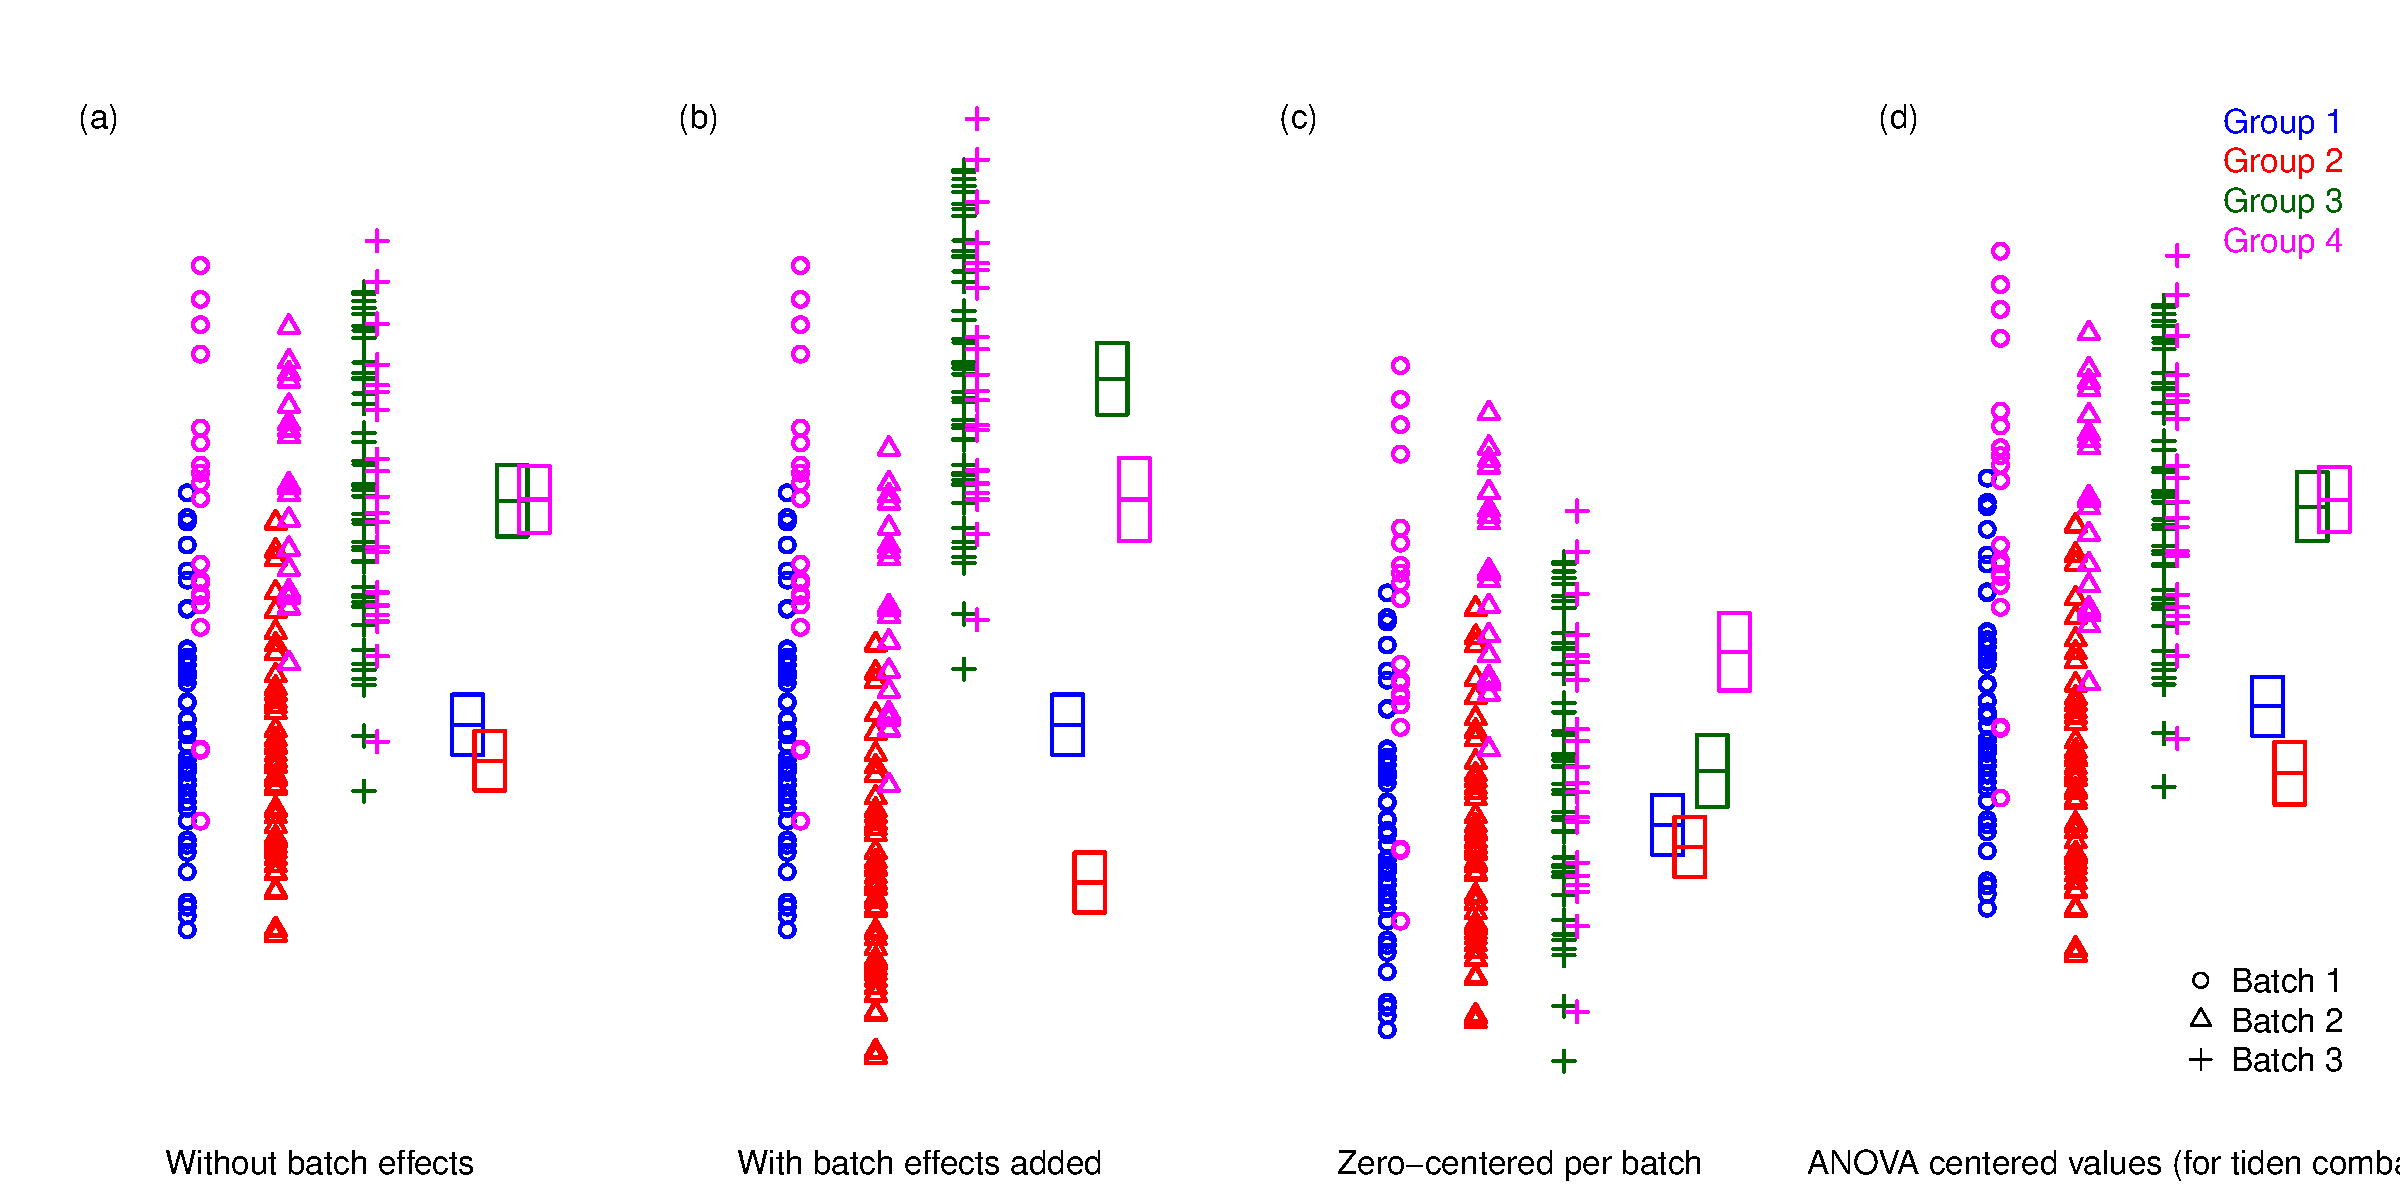
\includegraphics[width=13cm]{../figure1.pdf}
\caption{Simulated data from four study groups was generated where groups 1 and 2 have lower means than groups 3 and 4. These were placed in three different batches with batch effect added. Values and boxes showing mean and two standard errors of the mean are displayed for data without batch effects, after adding batch effects, after batch centering, and after ANOVA based batch centering. The last frame shows the least squares estimates of the group means from a two-way ANOVA analysis with 2 standard errors. This case, design and effects, was selected to illustrate the spurious effects that may arise.}
\label{fig:boxplots}
\end{figure}


\begin{figure}[!p]
\begin{center}$
\begin{array}{cc}
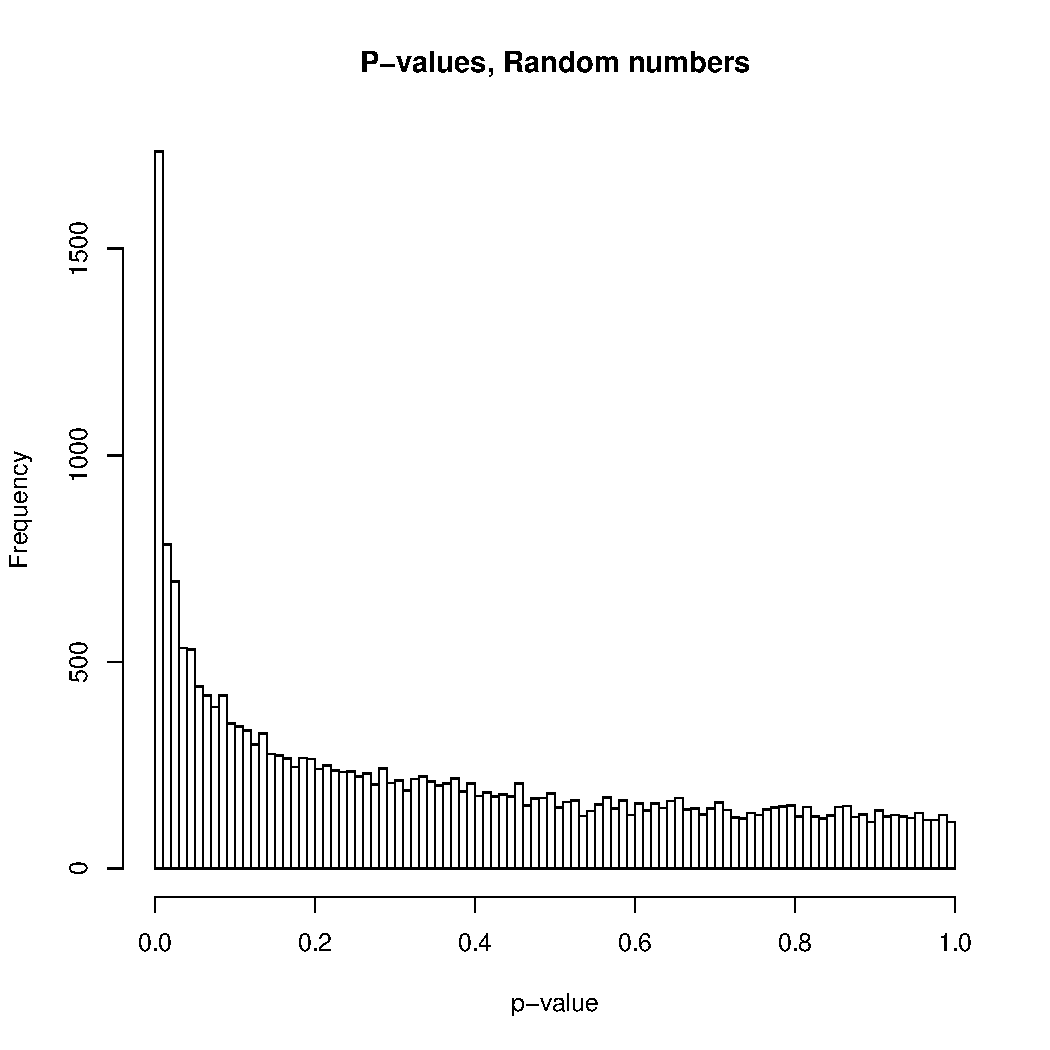
\includegraphics[width=6.5cm]{../reanalysis/Leek2012/leekrandomdatapvalues.pdf} &
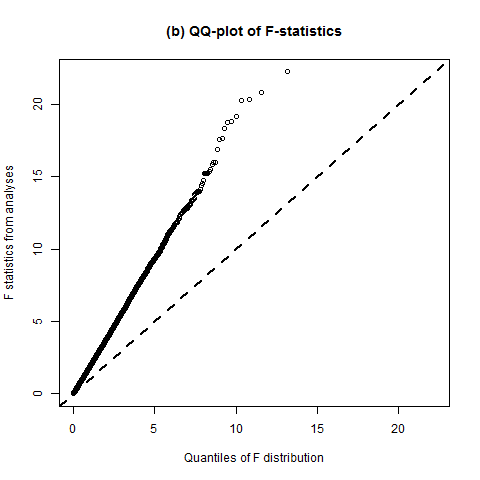
\includegraphics[width=6.5cm]{../reanalysis/Leek2012/leekqqplot.png}
\end{array}$
\end{center}
\caption
{
A sanity checks where the recommended use of ComBat fails. Adapted from the user guide in the sva package. Real data are substituted with random numbers from a normal distribution, but the batch-group design is retained. ComBat is applied followed by a F-test.
a) P-value distribution
b) QQ plot of the F-statistics
}
\end{figure}




\begin{figure}[!p]
\begin{center}$
\begin{array}{cc}
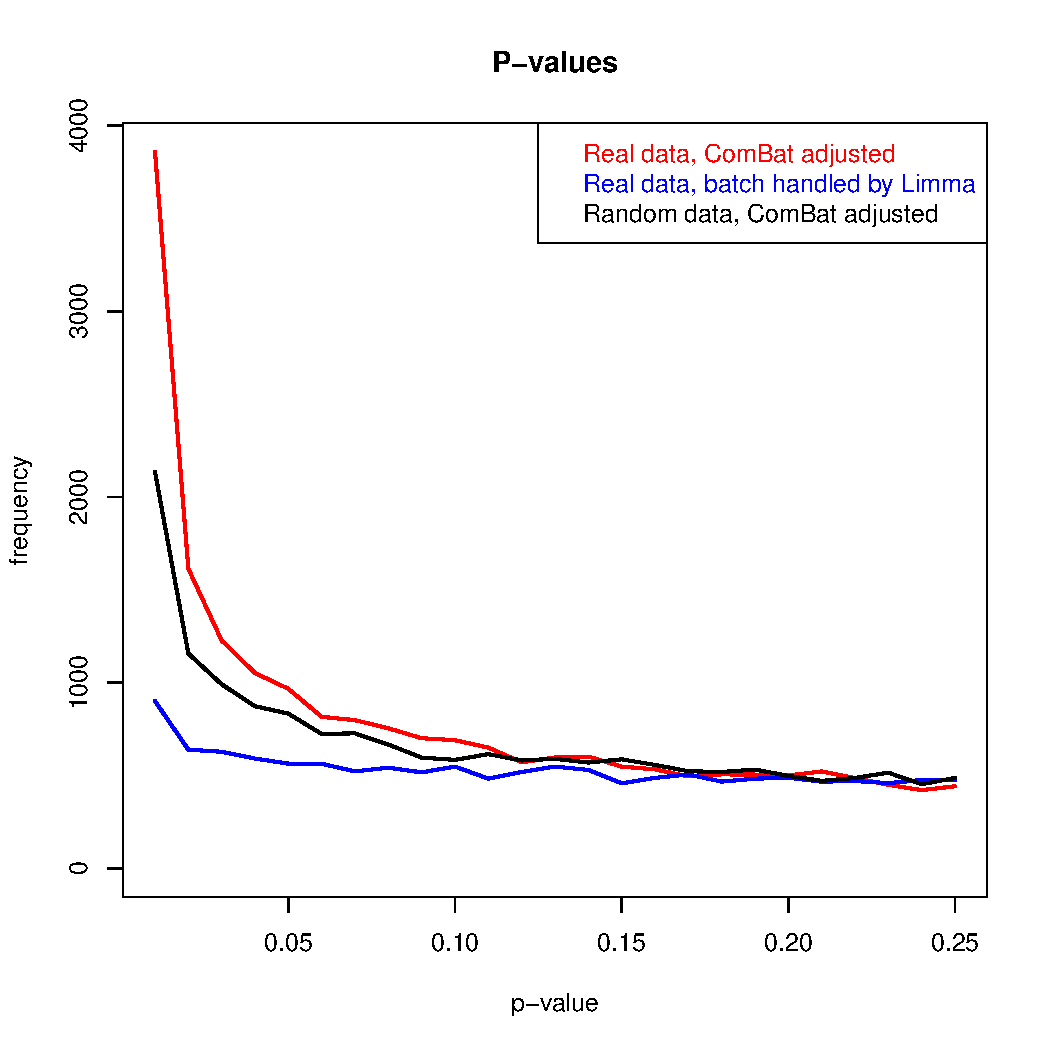
\includegraphics[width=6.5cm]{../reanalysis/Towfic2014/towficpvalues.pdf} &
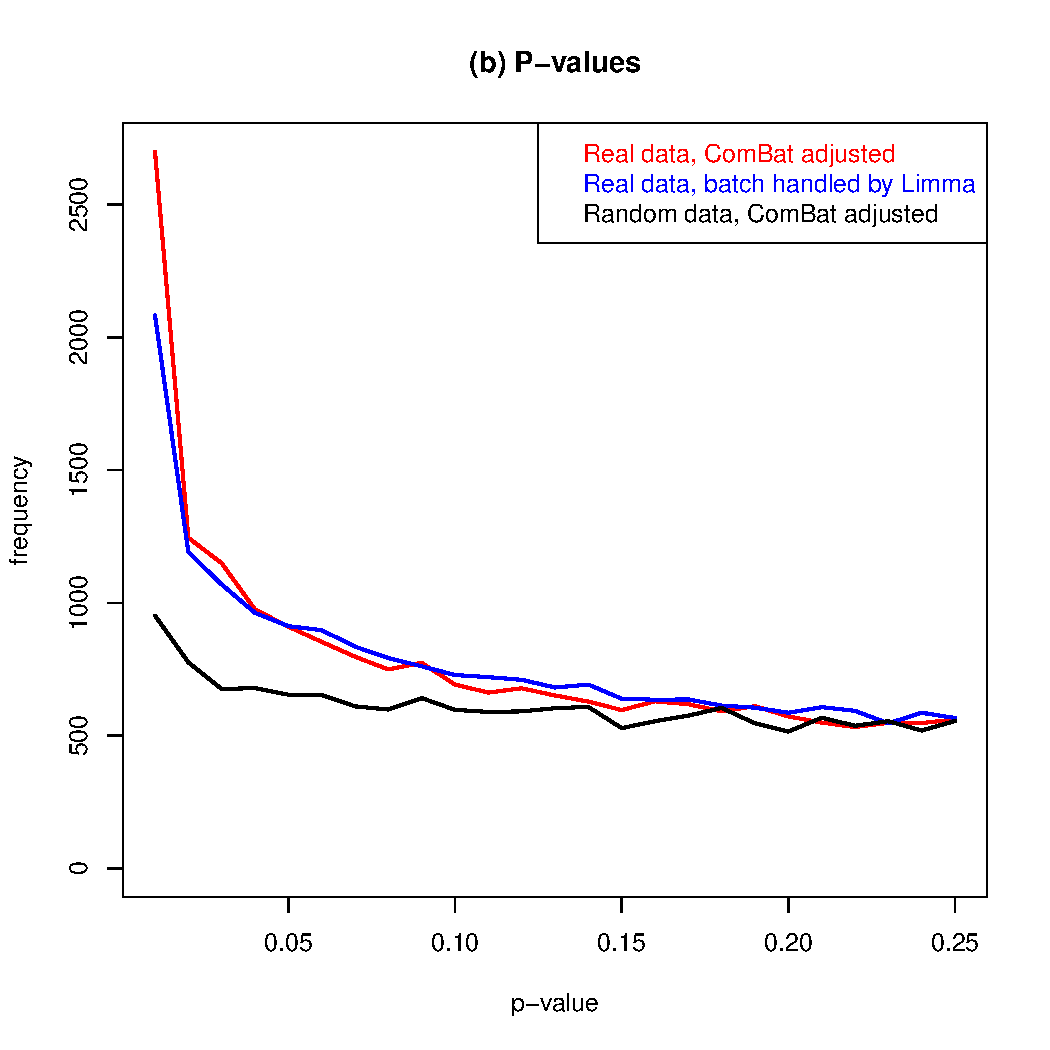
\includegraphics[width=6.5cm]{../reanalysis/Johnson2007/dataset2pvalues.pdf}
\end{array}$
\end{center}
\caption
{
Three analyses of two works where batch effects were adjusted for with ComBat. First as described in the original works with ComBat on real data. Secondly, with ComBat but with random numbers instead of real data. Thirdly without ComBat and instead blocking batch with limma on real data.
a) Re-analysis of  \citealp{Towfic2014}, glatiramer acetate vs. generic 
b) Re-analysis of "Data set 2" \citealp{Johnson2007},  TAL1 inhibition vs. control
}
\end{figure}



%\begin{table}[!p]
%\tblcaption{... \protect\citet{...} ... \label{Table1}}
%{\tabcolsep=4.25pt
%\begin{tabular}{@{}cccccccccc@{}}
%\tblhead{Dis & Chr & Marker & MLE-OR & MLE & MLE & EB-HM-OR & EB-HM & EB-HM & ES \\
%&&& (SE) & \textit{P}-value & rank & (SE) & \textit{P}-value & rank & rank}
%CAD & 2 & rs2943634 & 1.22(0.04) & $1.23 \times 10^{-5}$ & 32 & 1.02(0.01) & 0.19 & 28 & 37 \lastline
%\end{tabular}}
%\end{table}

\end{document}

